\documentclass[conference]{IEEEtran}
\usepackage{graphicx} % Required for inserting images
\usepackage{amsmath}
\usepackage{cite}
\usepackage{multirow}
\usepackage{fancyhdr}
\usepackage{subcaption}
\usepackage{booktabs}
\title{Exploring Unsupervised Learning and Dimensionality Reduction Algorithms: Weather and Housing Price Classification}
\author{Aditya Tomar \\ CS7641: Assignment 3 \\ atomar45@gatech.edu}

\fancypagestyle{fancy}{
    \fancyhf{} % clear all header and footer fields
    \fancyfoot[C]{\thepage} % page number in center of footer
}

\begin{document}

\maketitle

\begin{abstract}

\end{abstract}

\section{Introduction} Life is made up entirely of uncertainties. It has many ups and downs, as well as crests and valleys. However, it is our nature as humans to want to make sense of the world around us and find answers to how and why specific incidents happen. With so much to be aware of, it is easy to lose track of what problem we are trying to solve. To lessen the cognitive load, data scientists and machine learning engineers report their findings and put them into datasets and design models that can take this vast information and distill it to a compressed set of variables that capture the more valuable features in a process called dimensionality reduction to help us solve real-life problems and make sense of the world. Machine learning is the application of computational techniques to predict outcomes before they happen based on what has happened before, and there are two branches of this: Supervised and Unsupervised Learning. Assignment 1 explored how we can take our observations of the past (target variable) and see if the algorithm can recognize patterns and future outcomes. This assignment explores how we can use dimensionality reduction algorithms to identify and learn patterns in unlabeled data. 
\par This study aims to see if applying clustering to the datasets before they are reduced by the dimensionalilty reduction algorithms improves the neural networks performance rather than reducing it first and seeing if using the components created by PCA, ICA, and RP combined with KMeans and EM perform better than the Neural Network Learner from Assignment 1.
\par To investigate my hypotheses, I chose two datasets. One is the AMES Housing dataset, a classification problem containing many features like square footage, garage space, number of bathrooms, etc., factors that would help determine a home's fiscal value. The second is a time series dataset that contains meteorological data from numerous European cities over a year. 

\section{Step 1}
\par To determine the optimal number of clusters and components for clustering algorithms, I performed a quick EDA analysis on both the housing and weather datasets to see what were two important features of both datasets that I could use in my analysis. After standardizing the datasets using StandardScaler from the Scikit-Learn library, I created a correlation matrix including the target column to see what they top features were. I chose to use the average temperature and humidity characteristics from the weather data and the overall quality and size characteristics of the garage from the housing dataset. All these features showed a strong correlation with the target column from their respective datasets. I dropped those target columns to prepare for the implementation of KMeans and Expectation Maximization (EM) algorithms.
\par KMeans and EM are widely used clustering algorithms to analyze very noisy datasets and perform high dimensionality analysis. For my purposes, I will try to see how these clustering algorithms perform before any dimensional reduction. KMeans is very simple in how it assigns different data points to each cluster center and does well in cases where there is more rounder clusters. EM is a much more versatile variant and can handle irregular shaped clusters and non-normal distributions. I think I will see EM a much better candidate for the housing dataset as it has more complex distributions of features than KMeans.
\subsection{KMeans}
In both the weather and housing datasets, I created a function that could find the most optimal number of clusters for KMeans clustering. I implemented both the Elbow Method and the Silhouette Score Method as a way to compare k values derived from different approaches. 
\par The Elbow Method is a very straightforward approach as it is the sum of the squared distances between the datapoint and the centroid of the nearest cluster. You plot the sum of all the squared distances against different number of clusters. The elbow is just the point at which there is diminishing returns as you start adding more clusters. 
\par The Silhouette Method is more robust as you are trying to see how well matched each datapoint is to its respective cluster. The higher the value, the datapoints are well matched to their clusters, the lower the value it means datapoints are quite dissimilar to their own clusters we should find values for k that are smaller so that we maximize the silhouette score. 
\par Not only did the SS and Elbow Method return the same value on housing and weather data, but the value of clusters k was the same, 2. Since this was originally a binary classification problem having two clusters does make sense, it means that both datasets separate into two clusters naturally.
\begin{figure} 
    \centering
    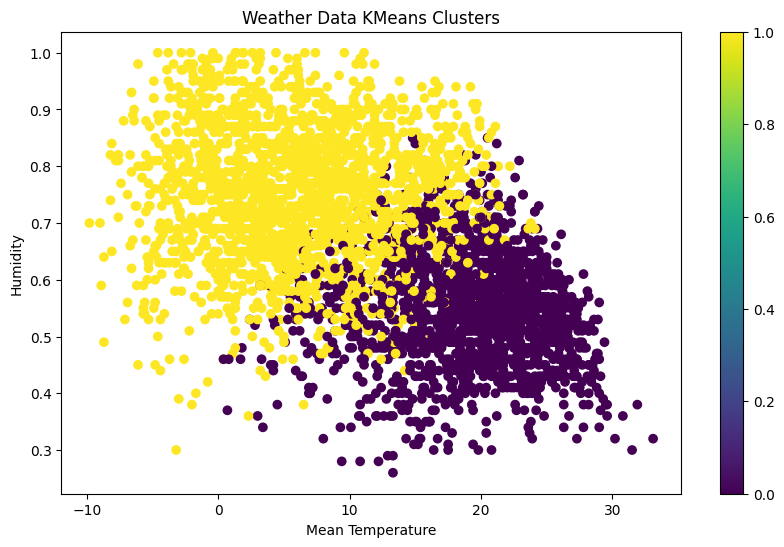
\includegraphics[width=1.0\linewidth]{figures//weather_figures/step_1a.png}
    \caption{Weather Data -- KMeans Clusters}
    \label{fig:1_weather_kmeans
}
\end{figure}
\par In Fig.1, we can see there is a clear separation between the classes for the mean temperature and humidity features. 
\begin{figure}
    \centering
    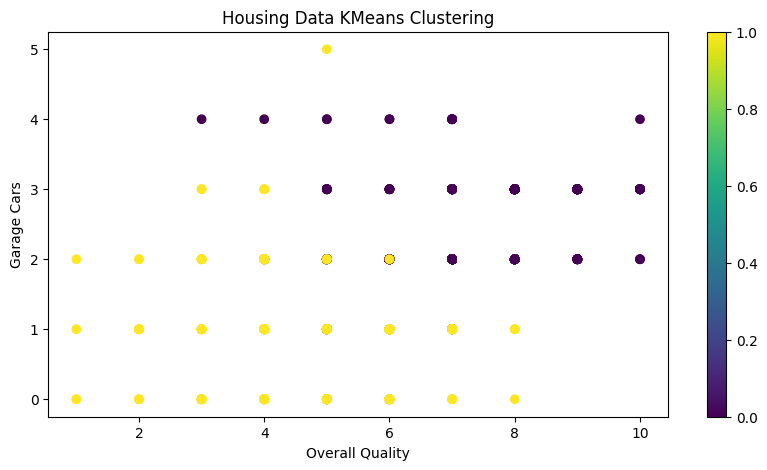
\includegraphics[width=1.0\linewidth]{figures//housing_figures/step_1c.png}
    \caption{Housing Data -- KMeans Clusters}
    \label{fig:2_housing_kmeans
}
\end{figure}
\par In Fig.2, we see something peculiar because the data is discrete and not continuous like the features in the weather data, we see this kind of dotted grid but can see a separation between the two.
\subsection{Expectation Maximization (EM)}
\par I used two methods as will to optimize the number components for the Gaussian Mixture Model I used for the EM method, the Akaike Information Criterion (AIC) and Bayes Information Criterion (BIC). From the lectures, I know that the BIC uses Bayes analysis to estimate the function of the posterior probability being true. It is better in cases where we have smaller datasets, so the models are not too complex. Akaike also penalizes parameters but it stresses the goodness of fit more, so it does not penalize the parameters too harshly. So it is better to use that optimization method for larger datasets and helps prevent overfitting because of the focus on goodness of fit. I wanted to compare how the different scoring affects the number of components for the EM method. Sure enough, it did not change much as both returned the same values n=10 and n=6.
\begin{figure}
    \centering
    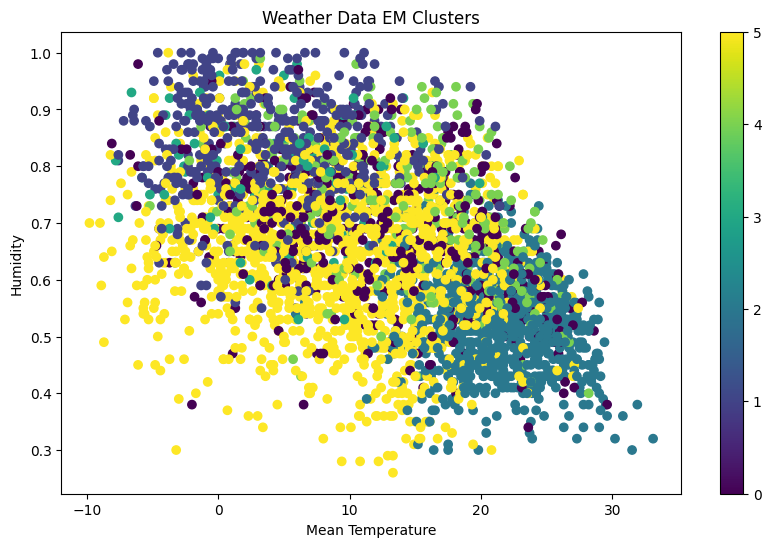
\includegraphics[width=1.0\linewidth]{figures//weather_figures/step_1b.png}
    \caption{Weather Data -- EM Components}
    \label{fig:3_weather_EM
}
\end{figure}
In Fig.3, we can see that the weather dataset has converged to 6 parameters. In Fig.4, the housing dataset converged to 10 parameters with clustering forming a similar grid like pattern to KMeans. 
\begin{figure}
    \centering
    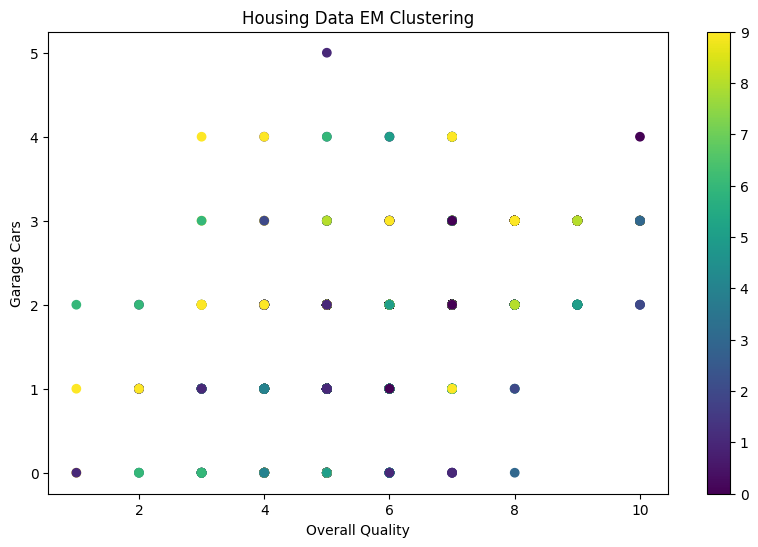
\includegraphics[width=1.0\linewidth]{figures//housing_figures/step_1d.png}
    \caption{Housing Data -- EM Components}
    \label{fig:4_housing_EM
}
\end{figure}
By the end of this step, I could see through different optimization methods for cluster values specialized in detecting goodness of fit and overfitting minimization, both datasets returned the same value, so it would seem that the datasets are properly scaled to move to the next step.
\section{Step 2}
Dimensionality Reduction is a very important for constructing unsupervised learning models for an unlabeled dataset and gives us the ability to streamline the data into its most important components. 
\subsection{Principal Component Analysis (PCA)}
\par PCA is a technique where original dataset is condensed to a set of uncorrelated components, and sorted by the amount of variance they have. It aims to retain as much variance as possible in few dimensions. Variance is important in PCA because it is the structure of the original dataset, without the dimension reduction becomes pointless if you lose too much information. To optimize to minimize loss in variance, I used the Explained Variance method to choose number of components based on the when the variance exceeds a certain threshold, in this case 95\%.
\par In both the housing and weather dataset, the cumulative variance increased with more components, adding to the total variance and then plateaued, suggesting earlier components had more importance overall, however I noticed a decreasing trend in the percentage of individual variance which suggests adding more components in fact does not add more importance if anything it leads to diminishing returns. Fig. 5 details the Explained Variance for the housing data.\\\\
\begin{figure}
    \centering
    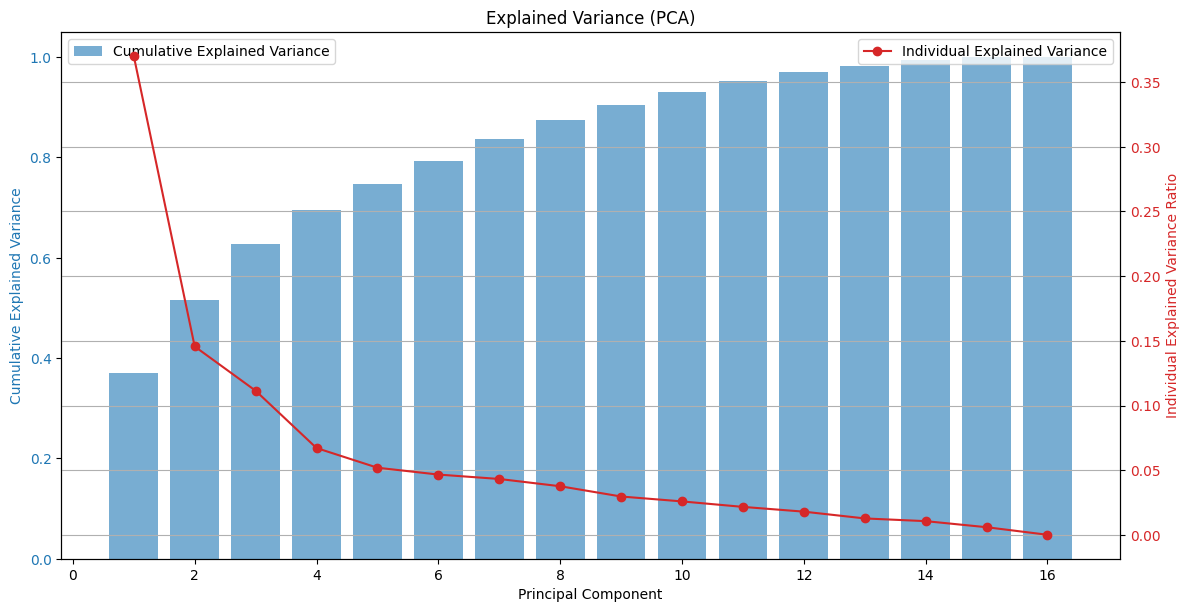
\includegraphics[width=1.0\linewidth]{figures//housing_figures/step_2a.png}
    \caption{Housing Data -- Explained Variance (PCA)}
    \label{fig:5_housing_ExpVariance
}
\end{figure}
\subsection{Independent Component Analysis (ICA)}
\par ICA is another alternative technique that identifies features that are independent from each other. Mainly used in signal processing to separate components from mixed signals. It tends to capture non-Gaussian structures in datasets, deviating from more symmetric, bell-shaped curves that you see in Gaussian distributions. ICA should be use when you have an array of independent sources that can be easily separated. I want to use ICA to see if we can reduce the dataset to include independent components. I used the Kurtosis method to find the optimal number of independent that both the weather and housing datasets have. 
\par Kurtosis is a measure that gives us the shape of the distribution of the data. In relation to ICA, it helps us it identify the features that are not normal in the data. In the graphs I was looking for where the value of kurtosis was the highest , meaning that the the data has outliers which makes it deviate from a bell shape normal distribution. Anywhere the data had lower kurtosis, this would tell me that for those number of components the data would be moving towards a normal distribution. So looking at Fig. 6 and Fig. 7, we see that kurtosis was maximized when the number of components were 8 and 3 respectively for the housing and weather datasets. 
\begin{figure}
    \centering
    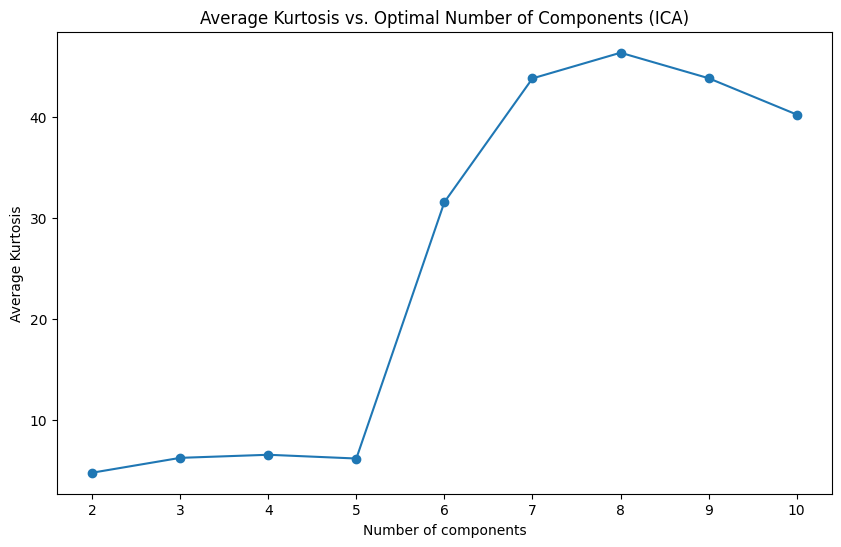
\includegraphics[width=0.9\linewidth]{figures//housing_figures/step_2b.png}
    \caption{Housing Data -- Kurtosis (ICA)}
    \label{fig:6_housing_kurtosis
}
\end{figure}
\begin{figure}
    \centering
    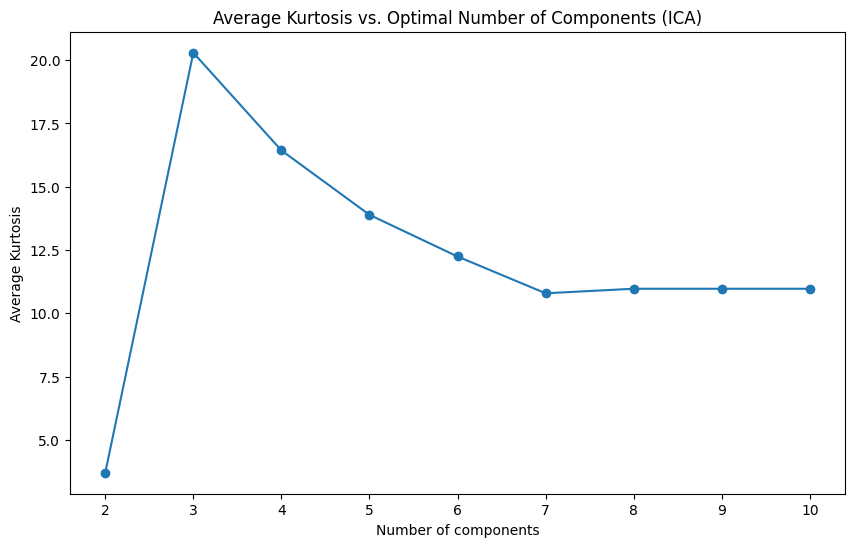
\includegraphics[width=0.9\linewidth]{figures//weather_figures/step_2c.png}
    \caption{Weather Data -- Kurtosis (ICA)}
    \label{fig:7_weather_kurtosis
}
\end{figure}
\subsection{Random Projection (RP)} 
\par Random Projection is the third dimensionality reduction method I used that uses a random matrix to project a higher dimensional data points onto a lower dimensional space. It is much faster than ICA and PCA in that it can project the entire dataset to a lower dimensional where as PCA involves calculating eigenvalues and eigenvectors and sorting them and ICA uses more complex mathematical operations to maximize the non-Gaussianity of the dataset. RP is straightforward operation where you multiply the matrix by some random matrix which is less intensive computationally. I used the Reconstruction error method to optimize the number of components. 
\par The Reconstruction Error method reconstructs the data from the lower dimensional space back to the original data, using an inverse matrix. The error calculation is just the difference between the original and reconstructed data. With the weather data in Fig. 8, I was looking to see where the reconstruction error reached the minimum, however, the error was still pretty high when I used reconstruction error method on the housing data. This makes sense that it performed poorly because it works better on larger datasets that need faster approximations, however with smaller datasets, it sacrifices accuracy for time complexity.
\par After looking at all three of these algorithms for dimensionality reduction on my datasets, I found that some algorithms perform better than others. In particular, ICA on the housing seemed to produce a decent amount of components. In the next step, I aim to take a closer look at the algorithms' clustering performance using different criterion and find the model-reduction combination that performed the best between the two datasets.
\begin{figure}
    \centering
    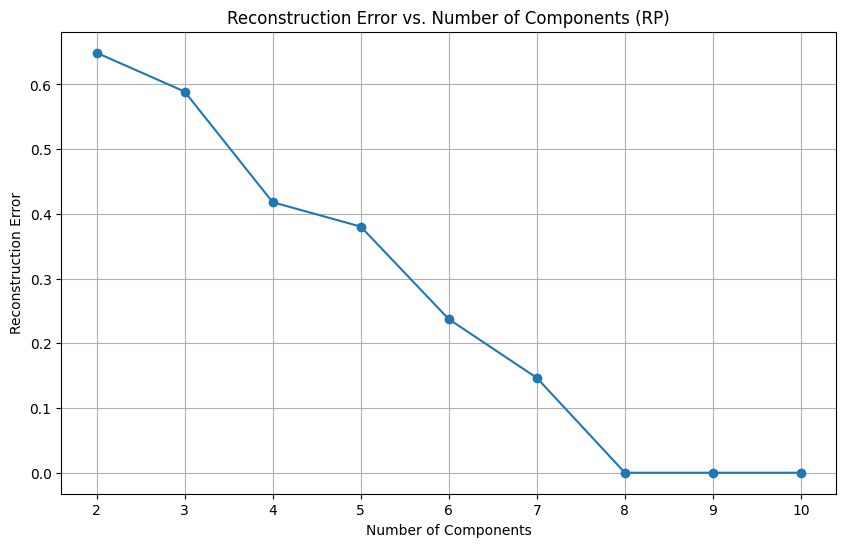
\includegraphics[width=0.9\linewidth]{figures//weather_figures/step_2d.png}
    \caption{Weather Data -- Reconstruction Error (RP)}
    \label{fig:8_weather_reconstruction
}
\end{figure}
\section{Step 3}
After applying the dimensionality reduction algorithms on my two datasets, there were many nuances and cases I had to consider in deciding the optimal values for the number of components for each algorithm. In this section, I want to compare and rank the different algorithm and model pairs across the two datasets to see which pair had the best performance using three scoring mechanisms.
\subsection{Silhouette Score}
\par As discussed in Step 1, Silhouette Method is a quite useful metric to use when trying to explore a data point's similarity with its assigned cluster and with other clusters too. The metric is also often used to identify how well-separated the clusters are. I mainly used the metric to assess how each model-algorithm pair handles the trade off between compactness and separation between the clusters.

\subsection{Davies-Bouldin Score}
\par The Davies-Bouldin Score is a metric that measures the mean similarity ratio of between two clusters. This metric is useful as it measures the inter-cluster scatter and intra-cluster separation, giving an insight into how well the model handled the clustering of the reduced data. To interpret the score, I am looking for lower values as it will indicate that the clusters are compact and are distinct, so there will clear separation.
\subsection{Calinski-Harabasz Score}
The Calinski-Harbasz Score or the Variance Ratio Criterion measures the relationship between the sum of intra-cluster and inter-cluster dispersion. This is also very useful in ranking our pairs because it also balances the compactness and separation of the clusters. A high score from this metric will indicate that the model had clustered the data well.
\section{Step 4}
\begin{table}[htp]
    \centering
    \caption{Performance Metrics for PCA, ICA, and RP}
    \label{tab:performance_metrics}
    \resizebox{\columnwidth}{!}{%}
    \begin{tabular}{lcccc}
    \toprule
    \textbf{Method} & \textbf{Accuracy} & \textbf{Training Time (s)} & \textbf{Prediction Time (s)} & \textbf{F1-Score Avg} \\
    \midrule
    \textbf{PCA} & 0.9334 & 3.4113 & 0.00041 & 0.93 \\
    \textbf{ICA} & 0.9471 & 2.6668 & 0.00051 & 0.95 \\
    \textbf{RP}  & 0.9181 & 2.1919 & 0.00032 & 0.92 \\
    \bottomrule
    \end{tabular}%
    }
\end{table}


\section{Step 5}

\begin{table}[htp]
    \centering
        \caption{Performance comparison of PCA, ICA, and RP with clusters.}
    \label{tab:performance_comparison}
      \resizebox{\columnwidth}{!}{%}
    \begin{tabular}{lcccc}
        \toprule
         \textbf{Method} & \textbf{Accuracy} & \textbf{Training Time (s)} & \textbf{Prediction Time (s)} & \textbf{F1-Score Avg} \\
        \midrule
        \textbf{PCA w/ Clusters} & 0.9454 & 3.6799 & 0.00038 & 0.95\\
        \textbf{ICA w/ Clusters} & 0.9369 & 3.55548 & 0.00029 & 0.94\\
        \textbf{RP w/ Clusters} & 0.9300 & 2.15453 & 0.00033 & 0.93\\
        \bottomrule
        
    \end{tabular}%
    }

\end{table}

\section{Conclusion}


\bibliographystyle{IEEEtran}
\begin{thebibliography}{1}

\bibitem{zenodo}
``A European daily high-resolution gridded meteorological data set for 1950–2021,'' accessed on: Jun. 9, 2024. [Online]. Available: https://zenodo.org/records/7525955

\bibitem{kaggle_weather}
``Weather Prediction Dataset,'' accessed on: Jun. 9, 2024. [Online]. Available: https://www.kaggle.com/datasets/thedevastator/weather-prediction

\end{thebibliography}

\end{document}
